\documentclass{beamer}

\mode<presentation> {
	\usetheme{CambridgeUS}
}

\usepackage[spanish]{babel}
\usepackage[utf8]{inputenc}
\usepackage{amsmath, amssymb}
\usepackage{hyperref}
\usepackage{geometry}
\usepackage{graphicx}
\usepackage{booktabs}
\usepackage{listings}

\title[\LaTeXe]{Introducción a la escritura científica en \LaTeX}

\author{Fernando Oleo Blanco}
\institute[ICAI]{
	\href{http://www.icai.comillas.edu/es/}{Universidad ICAI Comillas} \\
	Asociación de LinuxEC \\
	\medskip
	\textit{201507027@alu.comillas.edu}
}
\date{\today}

\begin{document}
	
\begin{frame}
	\titlepage 
\end{frame}

\begin{frame}
	\tableofcontents
\end{frame}

\section{Recursos}

\begin{frame}{Recursos recomendados}
	
	\begin{block}{Lectura}
		$\bullet$ \href{https://tobi.oetiker.ch/lshort/lshort.pdf}{\textit{The not so Short Introduction to \LaTeX}} por Tobias Oetiker. \\
		$\bullet$ \href{https://en.wikibooks.org/wiki/LaTeX}{\textit{\LaTeX\ Wikibook:}} Libro escrito por y para Wikipedia. \\
		$\bullet$ \href{http://osl.ugr.es/CTAN/info/Math_into_LaTeX-4/Short_Course.pdf}{\textit{More Math Into \LaTeX}} por George Grätzner (esta es una buena muestra).
	\end{block}
	\begin{block}{Internet}
		$\bullet$ \href{https://www.sharelatex.com/}{\textbf{Editor colaboratibo}} herramienta moderna para el trabajo en grupo, multiedición y tabajo a tiempo real en la nube. \\
		$\bullet$ \href{https://www.overleaf.com/}{\textbf{Overleaf:}} escritura de \LaTeX en el navegador $\leftarrow$ ya os estáis metiendo. \\
		$\bullet$ Cualquier servicio con plantillas (\href{http://www.latextemplates.com/}{\textbf{Latextemplates}} por ejemplo). \\
		$\bullet$ \href{https://www.tug.org/begin.html}{\textbf{Tug:}} Centro de recursos \textit{oficiales}. \\
		$\bullet$ \href{https://es.sharelatex.com/learn/}{Foros}, "puntos de información", etc. \\
		$\bullet$ Google.
	\end{block}
	
\end{frame}

\section{Razones}

\begin{frame}{¿Por qué?}
	\small \vspace{-6pt}
	\begin{block}{Rasgos generales}
		\begin{enumerate}
			\item Herramienta estándar de escritura científica. Prácticamente todos los servicios científicos tienen alguna herramienta de exportación.
			\item Gran flexibilidad. Fácil uso (más indicaciones a continuación).
			\item Muy buena integración con herramientas científicas: Matlab, Wolfram, R... y MS Word.
			\item Saber más nunca fue malo \tiny bueno... \small
		\end{enumerate}
	\end{block}
	\vspace{-6pt}
	\begin{block}{Características propias}
		\begin{enumerate}
			\item Fácil lectura.
			\item Estructuración y formalidad absoluta.
			\item Eficiente en la escritura.
			\item Perfectamente integrado en el texto.
			\item Requiere de un largo aprendizaje, pero prisa no hay.
		\end{enumerate}
	\end{block}
\end{frame}

\section{Introducción general}

\begin{frame}{Otra introducción a \LaTeX}
	Ya que muchos no sabéis absolutamente nada de \LaTeX... Vuelta a la introducción. \\
	\begin{block}{TexStudio}
		$\bullet$ \href{http://www.texstudio.org/}{\textbf{\TeX Studio:}} Download $\rightarrow$ busca tu plataforma. Instálalo como solo tú sabes.
	\end{block}
	
	\begin{block}{TexLive}
		$\bullet$ \href{https://www.tug.org/texlive/}{\textbf{Tug}} \\
		Windows: pincháis en download e instaláis, instaláis \textbf{todo} 4.5Gb \\
		Mac: Link MacTeX distribution. Instaláis y listo. \\
		Linux y BSD: ya sabéis.
	\end{block}	
\end{frame}

\begin{frame}[fragile]{Consejos}
	Procedimiento que \textbf{simpre, siempre, siempre} seguiréis:
	\begin{itemize}
		\item Nunca empecéis desde un documento en blanco, usad plantillas (templates).
		\item Crearos vuestras propias plantillas.
		\item Usad comentarios, especialmente si acabáis de empezar \verb|% comentario|.
		\item No compliques demasiado las cosas, como en programación, con \texttt{for} se hace mucho, solo hay que jugar con él.
		\item Google.
		\item Acordaros que funciona como un entorno de programación.
	\end{itemize}
\end{frame}

\begin{frame}[fragile]{Estructura básica de un comando}
	\vspace{-8pt}
	\begin{block}{Comando normal}
		Ejemplo: \verb|\documentclass[12pt, landscape, a4paper]{article}|
		Las partes son:
		\begin{itemize}
			\item El propio comando \verb|\documentclass|
			\item Las opciones de uso de ese comando \verb|[12pt, landscape, a4paper]|.
			\item Y los datos de ese comando (argumento) \verb|{article}|
			\item De lo anterior puede que sean opcionales u obligatorias las opciones y/o el argumento.
		\end{itemize}
	\end{block}
	\begin{block}{Comando de entorno}
		E.j: \verb|\begin{columns}[T] ... \end{columns}| y \verb|\begin{block}{Argumento del entorno} ... \end{block}| \\
		El mismo cuento. Pero hay que añadir el detalle de que el entorno se pone entre llaves después de \verb|\begin|.
	\end{block}
\end{frame}

\begin{frame}[fragile]{Documento básico en \LaTeX}
	\begin{columns}[T]
		\column{.4\textwidth}
		\vspace{-12px}
		\begin{verbatim}
		\documentclass[]{article}
		
		\title{}
		\author{}
		
		\begin{document}
		
		\maketitle
		
		\section{}
		
		\end{document}
		\end{verbatim}
		\column{.6\textwidth}
		Ha de estar siempre, define nuestro trabajo \\
		\vspace{13px}
		Nuestra información personal \\
		\vspace{29px}
		Aquí comienza nuestro documento \\
		\vspace{13px}
		Nos hace nuestra portada automáticamente \\
		\vspace{13px}
		Una sección (parte principal del texto) \\
		\vspace{13px}
		Finaliza nuestro trabajo
	\end{columns}
\end{frame}

\begin{frame}[fragile]
	Los de habla española tenemos que configurar nuestro documento un poco. Aunque \TeX\ se diseñase hasta para aceptar chino, no lo usa por defecto. Además, tiene sus ventajas. A continuación de \verb|\documentclass[]{article}| vamos a poner las siguientes líneas:
	\begin{itemize}
		\item \verb|\usepackage[utf8]{inputenc}|
		\item \verb|\usepackage[spanish]{babel}|
		\item \verb|\usepackage{graphicx}|
		\item \verb|\usepackage{amsmath, amssymb}|
		\item \verb|\usepackage{hyperref}|
		\item \verb|\usepackage{geometry}|
	\end{itemize}
	Los dos primeros son para que nos deje poner la Ñ y parta las palabras con guión de manera correcta (99\% de los casos) de manera automática. ¿A que mola? \texttt{Graphicx} para poner fotos; \texttt{Amsmath} para símbolos matemáticos y mucho más. \texttt{Geometry} para cambiar las dimensiones de los márgenes. \texttt{Hyperref} para hacer referencias externas e internas.
\end{frame}

\begin{frame}[fragile]{Comandos de estructura}
	\begin{block}{}
		\begin{itemize}
			\item \verb|\include{file}| Incluir otro texto escrito en \texttt{.tex}
			\item \verb|\tableofcontents| Genera índices de manera automática con los comandos que vienen a continuación.
			\item \verb|\chapter{title}| Solo disponible en \verb|book|.
			\item \verb|\section{title}| Parecido a \verb|\chapter| pero utilizable en cualquier entorno (En Beamer funciona distinto).
			\item \verb|\subsection{title}| y \verb|\subsubsection{title}|.
			\item \verb|\paragraph{text}| Párrafos especiales (no apaerecen en el índice).
		\end{itemize}
	\end{block}
	El uso y configuración de \verb|\makeindex| queda fuera de esta charla \\
	\textbf{Nota:} en este recuadro no he puesto título, fíjate en la diferencia.
\end{frame}

\begin{frame}[fragile]{Márgenes}
	Los márgenes en \LaTeXe\ son diseñados para escritura profesional, no son sencillos de manejar. Tendremos que usar las opciones del paquete \texttt{Geometry.} \\
	Como se indico anteriormente usaremos el comando \verb|\geometry{options}| con sus argumentos para definir los márgenes queridos. Unos márgenes sanos y de fácil modificación son los siguiente. \\~
	
	\verb| \geometry{|
	\verb|a4paper,|
	\verb|total={170mm,257mm},|
	\verb|left=20mm,|
	\verb|top=20mm,|\} \\~
	
	Más información en \href{https://www.sharelatex.com/learn/Page_size_and_margins}{\textcolor{blue}{Share\LaTeX}}
\end{frame}

\begin{frame}[fragile]
	\begin{block}{Items}
		\verb|\begin{itemize}| \\
		\verb|\item[label] description| \\
		\verb|\end{itemize}| 
	\end{block}
	\begin{block}{Enumerate}
		\verb|\begin{enumerate}| \\
		\verb|\item[label] description| \\
		\verb|\end{enumerate}|
	\end{block}
	\begin{block}{Notas a pie de página}
		Esto es un poco de texto.\footnote{Y esto la anotación} Y este mejor\footnote[frame]{¿A que sí?}. \\
		
		\verb|Esto es un poco de texto.\footnote{Y esto la anotación}| \\
		\verb|Y este mejor\footnote[frame]{¿A que sí?}|
	\end{block}
\end{frame}

\begin{frame}{Donald Ervin Knuth}
	\vspace*{-15pt}
	\begin{figure}
		\centering
		\vspace*{10px}
		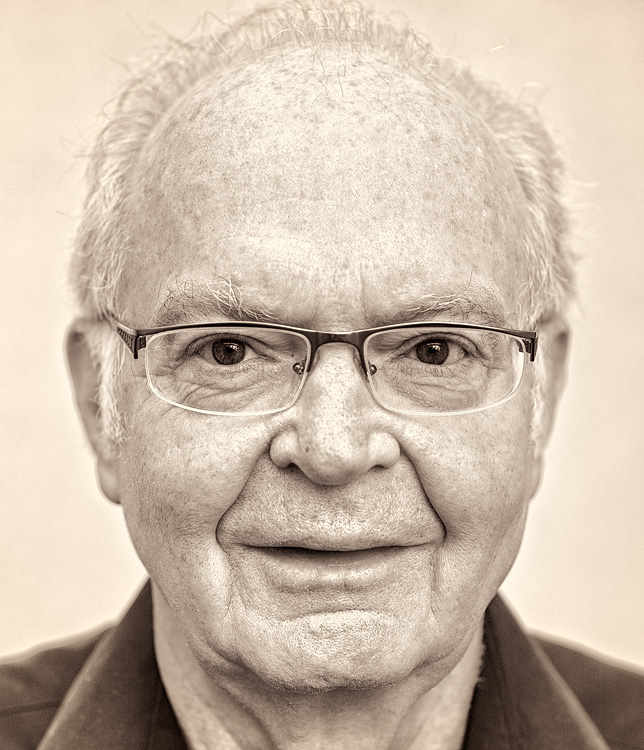
\includegraphics[height=0.55\linewidth]{images/Donald-Knuth-Stanford-Computer-Science}
		\caption{Donald Ervin Knuth. Creador de \TeX}
		\label{fig:donald-knuth-stanford-computer-science}
	\end{figure}
\end{frame}

\section{Introducción cualitativa}

\begin{frame}{Desarrollo y lógica del comando}
	\small Pudiendo daros un montón de datos no sería útil, así que continuemos con las herramientas.
	\begin{block}{Creación y diseño}
		\LaTeX\ fue creado por un matemático bien pragmático, que también es considerado uno de los padres de la informática moderna, siendo su especialidad el \textbf{diseño} de algoritmos. \LaTeX\ se creó para ser una herramienta eficiente y flexible que solucionara los problemas presentes de la tipografía y de la escritura científica; además de ser estable (seguimos con la misma versión desde 1994 de \TeX).
	\end{block}
	\begin{block}{Mnemotecnia}
		Una herramienta que requiera más tiempo para poder ser utilizada que para trabajar no tiene ningún sentido, \LaTeX\ soluciona tal problema (sorprendente). Para facilitar su uso, su diseño es puramente mnemotécnico y gráfico, a la vez que expresivo. Aprender su diseño es cuestión de hora y media.
	\end{block}

\end{frame}

\begin{frame}[fragile]{Comenzamos}
	Notas importantes en la lógica de la escritura científica en \LaTeX:
	\begin{block}{Desarrollo}
		$\bullet$ \LaTeX\ se creó para permitir una fácil y rápida creación de textos, aunque parezca poco intuitivo al principio. \\
		\textbf{Regla de la mano derecha:} si algo es muy utilizado y básico en el mundo de las matemáticas y de las ciencias, está acortado, simplificado. El resto son los nombres descriptivos. \textbf{Ejemplo:} la integral cerrada se usa mucho $\rightarrow$ está simplificada: $$\oint = \verb|$\oint$|$$ La doble integral cerrada sigue su desarrollo, pero no viene en Amsmath: \verb|$\oiint$|. La flecha a la derecha no es un símbolo matemático muy querido $\rightarrow$ no se abrevia \verb|$\rightarrow$|
	\end{block}
\end{frame}

\begin{frame}[fragile, plain]{Y continuamos}
	\small En \LaTeX\ existen dos formas de escribir fórmulas matemáticas. La razón es simple, estilo y formato. Estos dos modos son \textbf{Inline} y \textbf{Display}.
	\begin{block}{Inline}
		Traducido al español: en línea. Se usa para meter símbolos y fórmulas \textbf{dentro del texto.} Este modo respetará el formato que posea el texto. Se accede con el signo del dólar, todo lo que caiga dentro, estará en modo \textbf{Inline.} Ejemplo: $\frac{2^2}{4} = 1$ \verb|$\frac{2^2}{4} = 1$|, \verb|\(...\)| también se permite.
	\end{block} \pause
	\begin{block}{Display}
		Traducción: demostración. Se utiliza para la escritura a parte de la expresión matemática, por ejemplo, para grandes ecuaciones, fórmulas importantes o elementos grandes (matrices). Genera un espacio nuevo para la fórmula. Se accede desde entornos o con la siguiente secuencia: \verb|\[...\]|. Como ejemplo: \[\frac{2^{23}}{4} = 2^{21}\] \verb|\[\frac{2^{23}}{4} = 2^{21}\]|.
	\end{block}
\end{frame}

\section{Un poco de simbología y ejemplos}

\begin{frame}[fragile]
	\begin{block}{Alfabeto griego}
		Es especialmente expresivo, lo cual ayuda bastante a la hora de leer el código:
		\begin{columns}[onlytextwidth]
			\begin{column}{0.25\textwidth}
				\begin{equation*}
					\begin{split}
					\alpha \\
					\beta \\
					\gamma \\
					\varpi
					\end{split}
				\end{equation*}
			\end{column}
			\begin{column}{0.25\textwidth}
				\begin{verbatim}
					\alpha 
					\beta 
					\gamma 
					\varpi
				\end{verbatim}
			\end{column}
			\begin{column}{0.25\textwidth}
				\begin{equation*}
					\begin{split}
					\Gamma \\
					\Delta \\
					\varDelta \\
					\Sigma
					\end{split}
				\end{equation*}
			\end{column}
			\begin{column}{0.25\textwidth}
				\begin{verbatim}
					\Gamma 
					\Delta 
					\varDelta
					\Sigma
				\end{verbatim}
			\end{column}
		\end{columns}
	\end{block}
	\begin{block}{Y algún símbolo matemático}
		\vspace{-15pt}
		\begin{columns}[onlytextwidth]
			\begin{column}{0.1\textwidth}
				\begin{equation*}
					\footnotesize\begin{split}
					\pm \\
					\circ \\
					\iiint \\
					\sum \\
					\prod
					\end{split}
				\end{equation*}
			\end{column}
			\begin{column}{0.15\textwidth}
				\begin{verbatim}
				\pm 
				\circ 
				\iiint 
				\sum 
				\prod
				\end{verbatim}
			\end{column}
			\begin{column}{0.1\textwidth}
				\begin{equation*}
				\begin{split}
					\neq \\
					\equiv \\
			 		\approx \\
					\geq \\
					\propto
				\end{split}
				\end{equation*}
			\end{column}
			\begin{column}{0.15\textwidth}
				\begin{verbatim}
				\neq 
				\equiv
				\approx
				\geq 
				\propto
				\end{verbatim}
			\end{column}
			\begin{column}{0.15\textwidth}
				\begin{equation*}
				\begin{split}
					\rightarrow \\
				\Longrightarrow \\
				\Longleftrightarrow \\
				\overbrace{abc} \\
				\overrightarrow{abc}
				\end{split}
				\end{equation*}
			\end{column}
			\begin{column}{0.35\textwidth}
				\begin{verbatim}
				\rightarrow 
				\Longrightarrow 
				\Longleftrightarrow 
				\overbrace{abc} 
				\overrightarrow{abc}
				\end{verbatim}
			\end{column}
		\end{columns}
	\end{block}
\end{frame}

\begin{frame}[fragile]{Un par de ecuaciones para que os familiaricéis}
	\begin{block}{Ecuación de Bernoulli}
	\[ \left(\frac{p}{\rho g} + \frac{\alpha}{2g}V^2 + z\right)_{ent} = \left(\frac{p}{\rho g} + \frac{\alpha}{2g}V^2 + z\right)_{sal} + h_{tur} + h_{fr} - h_{bom} \]
	
	\small \verb|\[ \left(\frac{p}{\rho g} + \frac{\alpha}{2g}V^2 + z\right)_{ent}| \\ \verb| = \left(\frac{p}{\rho g} \frac{\alpha}{2g}V^2 + z\right)_{sal}| \\ \verb|+  + h_{tur} + h_{fr} - h_{bom} \]| \normalsize
	\end{block}
	\begin{block}{Hermosas mates}
		\[ \zeta(s) = \sum\limits_{n=1}^{\infty}\frac{1}{n^s} \qquad \Gamma(z) = \int_{0}^{\infty} t^{z-1} e^{-t} dt\]
		\verb|\[ \zeta(s) = \sum\limits_{n=1}^{\infty}\frac{1}{n^s} \qquad| \verb|\Gamma(z) = \int_{0}^{\infty} t^{z-1} e^{-t} dt\]|
	\end{block}
\end{frame}

\section{Tablas}

\begin{frame}[fragile]{Tablas}
	\begin{block}{Entorno tabular/array básico}
		Esto es la introducción básica general. \textbf{Nota:} las opciones de alineación son obligatorias.
		\verb|\begin{tabular}{alineaciones} ... \end{tabular}|
	\end{block}
	Ejemplo: 
	\begin{tabular}{l||c|r}
		11            &  12   &            13 \\
		\hline\hline
		hola          & hola  &          hola \\
		\hline
		adiós querida & adiós & Sayonara Baby
	\end{tabular}
	\begin{block}{}
		\begin{verbatim}
		\begin{tabular}{l||c|r}
		11            &  12   &            13 \\
		\hline \hline
		hola          & hola  &          hola \\
		\hline
		adiós querida & adiós & Sayonara Baby
		\end{tabular}
		\end{verbatim}
	\end{block}
\end{frame}

\subsection{Matrices}

\begin{frame}[fragile]{Matrices}
	Como las tablas, son fácilmente modificables:
	\begin{block}{Arrays}
		Funciona igual que el entorno tabular pero se usa dentro del entorno de escritura matemática. Juntando esto con el \verb|\left(...\right)| o cualquier otro símbolo podemos hacer matrices.
	\end{block} \pause
	\begin{block}{Pero \LaTeX\ es bien eficiente}
		Las matrices son una herramienta bien usada, por lo que hay una forma sencilla. \verb|\begin{*matrix}...\end{*matrix}|. No requiere de opciones de alineación. \textbf{*:} significa el tipo de puntuación a usar: \textbf{p:} paréntesis; \textbf{v:} vertical; \textbf{b:} corchetes; \textbf{B:} llaves. \textbf{Ejemplo:}
		\[\begin{pmatrix}
		1 & 2 \\
		3 & 4
		\end{pmatrix} \rightarrow 
		\begin{vmatrix}
		1 & 2 \\
		3 & 4
		\end{vmatrix} = -2 \Rightarrow 
		\begin{bmatrix}
		1 & 2 \\
		3 & 4
		\end{bmatrix}^2 = 
		\begin{bmatrix}
		7 & 10 \\
		15 & 22
		\end{bmatrix}\]
	\end{block}
\end{frame}

\begin{frame}[fragile]{El ejemplo de las matrices}
	\small
	\begin{verbatim}
		\[\begin{pmatrix}
		1 & 2 \\
		3 & 4
		\end{pmatrix} \rightarrow 
		\begin{vmatrix}
		1 & 2 \\
		3 & 4
		\end{vmatrix} = -2 \Rightarrow 
		\begin{bmatrix}
		1 & 2 \\
		3 & 4
		\end{bmatrix}^2 = 
		\begin{bmatrix}
		7 & 10 \\
		15 & 22
		\end{bmatrix}\]
	\end{verbatim} \normalsize
\end{frame}

\section{Ecuaciones}

\begin{frame}[fragile]{Entorno equation(*)}
	\begin{block}{La base de la estructuración}
		\verb|\begin{equation}...\end{equation}| tiene los mismos efectos que \verb|\[...\]| sin embargo, para ecuaciones formales, importantes y largas es preferido. Da mayor claridad al código, otros entornos se pueden usar dentro suyo y permite la \textbf{referencia y numeración.} Para evitar la numeración se le pone un * al final de su declaración. La \textbf{numeración} puede modificarse para que tenga en cuenta el capítulo, sección, etc.
	\end{block} \pause
	\begin{block}{Ejemplo}
		\begin{equation} \label{ec:ejemplo1}
			 f(x)=(x+a)(x+b)
		\end{equation}
		Como se puede ver en \ref{ec:ejemplo1}, escribir en \LaTeX\ es bien sencillo. \small
		\begin{verbatim}
			\begin{equation} \label{ec:ejemplo1}
			f(x)=(x+a)(x+b)
			\end{equation}
		\end{verbatim} \normalsize
	\end{block}
\end{frame}

\begin{frame}[fragile]{Desarrollando un poco más el tema...}
	\begin{block}{Subequations}
		Permite numerar distintas ecuaciones dentro de un mismo entorno y separación de las mismas. También permite cierta alineación.
	\end{block} \pause
	\begin{block}{Align}
		\textbf{Entorno muy querido y usado.} Permite partir largas ecuaciones en diferentes líneas. Se usa mucho para demostraciones, ya que estas requieren un gran número de pasos e igualdades, por lo que se suelen partir en diferentes líneas. Numera cada nueva ecuación, por lo que se suele usar (*). Si solo se quiere un número, se suele usar \textit{split o aligned} o la opción \verb|\nonumber| \textbf{Ejemplo:}
		\vspace{-15pt}
		\begin{columns}
			\column{0.5\textwidth}
			\begin{align}
			f(x) &= (x+a)(x+b) \\
			&= x^2 + (a+b)x + ab
			\end{align}	
			\column{0.5\textwidth}
			\begin{verbatim}
			\begin{align}
			f(x) &= (x+a)(x+b) \\
			&= x^2 + (a+b)x + ab
			\end{align}
			\end{verbatim}
		\end{columns}
	\end{block}
\end{frame}

\section{Recursos expresivos}

\begin{frame}[fragile]{Más flexibilidad en la escritura}
	\LaTeX\ es conocido por ser muy formal, lo que puede echar atrás a entusiastas de las anotaciones sobre el texto, correcciones anotadas etc. \LaTeX\ no trae herramientas sencillas que hagan esta labor de manera bonita, pero podemos jugar con lo que tenemos.
	\begin{block}{Anotaciones sobre fórmulas}
		\begin{itemize}
			\item \verb|\overset{}{} y \underset{}{}| Nos permiten poner unos símbolos encima de otros. Ejemplo:  $A \overset{!}{=} B; A \stackrel{!}{=} B \rightarrow$ \verb|$A \overset{!}{=} B; A \stackrel{!}{=} B$|. \pause
			\item \verb|\overbrace{} y \underbrace{}| Nos permiten coger trozos de ecuaciones. Ejemplo: $z = \overbrace{ \underbrace{x}_\text{real} + \underbrace{iy}_\text{imaginario} }^\text{número complejo} \rightarrow$ \small \verb|$z = \overbrace{\underbrace{x}_\text{real} +| \verb|\underbrace{iy}_\text{imaginario}}^\text{número complejo}$| \normalsize
		\end{itemize}
	\end{block}
\end{frame}

\begin{frame}[fragile]{Tipografía}
	\Large Fuentes
	\begin{itemize}
		\item \verb|\mathbb{}:| $\mathbb{SOLO \; MAY\acute{U}SCULAS}$
		\item \verb|\mathbf{}| $\mathbf{1234 \quad text}$
		\item \verb|\mathfrak{}| $\mathfrak{1234 \quad text \quad Re, Z, L, F, N}$
		\item \verb|\mathrm{}| $\mathrm{1234 \quad text}$
		\item \verb|\mathcal{}| $\mathcal{SOLO \; MAY\acute{U}SCULAS}$
		\item \verb|\mathrm{}| $\mathsf{1234 \quad text}$
		\normalsize
	\end{itemize}
\end{frame}

\begin{frame}[fragile]{Cuadros}
	\begin{block}{Solo ecuación}
		\verb|\begin{equation} \boxed{f(x)=(x+a)(x+b)} \end{equation}|
	\begin{equation}
		\boxed{f(x)=(x+a)(x+b)}
	\end{equation}
	\verb|\fbox{\begin{equation} f(x)=(x+a)(x+b) \end{equation}}|
	\end{block}	
	\begin{block}{Toda la ecuación}
		\fbox{\begin{minipage}{\linewidth}
			\begin{equation}
				f(x)=(x+a)(x+b)
			\end{equation}
		 \end{minipage}}
	\begin{verbatim}
		\fbox{\begin{minipage}{\linewidth}
		\begin{equation}
		f(x)=(x+a)(x+b)
		\end{equation}
		\end{minipage}}
	\end{verbatim}
	\end{block}
\end{frame}

\begin{frame}[fragile]{Referencias}
	Aunque no es un procedimiento único al apartado científico, hacer referencias es prácticamente una necesidad. \\~
	Aquí es donde \LaTeX\ brilla de nuevo, ya que automatiza el proceso \textbf{independientemente del contenido.} Las referencias tienen dos partes.
	\begin{block}{Label}
		\verb|\label{key}| Es el comando con el que etiquetamos un contenido, ya sean párrafos, ecuaciones, imágenes, etc. \texttt{key} será el \textit{código}, la etiqueta que nosotros le pondremos a nuestra referencia para luego llamarla cuando sea necesario.
	\end{block}
	\begin{block}{Reference}
		\verb|\ref{text}| Nos permitirá llamar a nuestra referencia donde sea necesario. Solo tenemos que introducir el \textit{código} para que la referencia sea creada.
	\end{block}
	\textbf{Ejemplo:} Véase la primera ecuación \ref{ec:ejemplo1}.	
\end{frame}

\begin{frame}[fragile]{Imágenes}
	\begin{block}{Imágenes}
		\begin{verbatim}
		\begin{figure}
		\centering
		\vspace*{10px}
		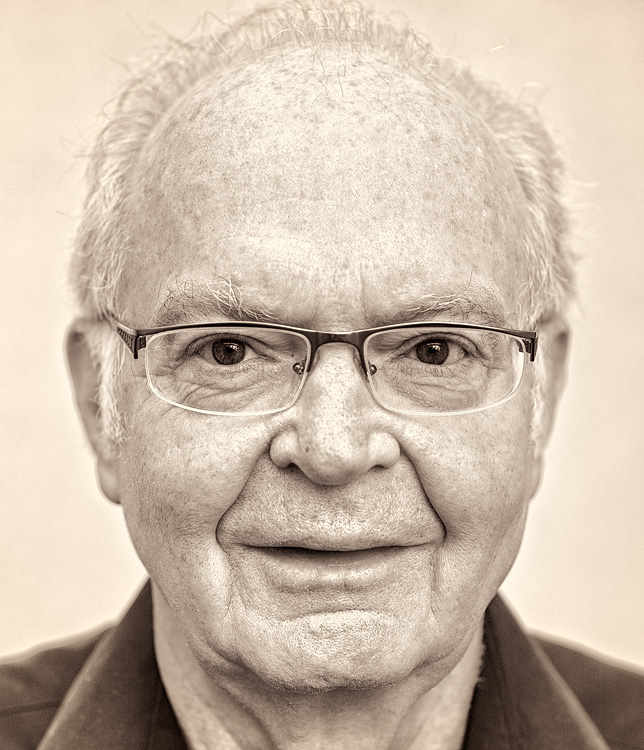
\includegraphics[height=0.6\linewidth]{images/Donald-Knuth-Stanford-Computer-Science}
		\caption{Donald Ervin Knuth. Creador de \TeX}
		\label{fig:donald-knuth-stanford-computer-science}
		\end{figure}
		\end{verbatim}
	\end{block}
	\begin{block}{}
		$\bullet$ \verb|\includegraphics[keyvals]{imagefile}| [Keyvals] son los valores de tamaño; se está haciendo aritmética, se esta cogiendo el 0.6 de todo el tamaño de línea. \{Dirección relativa a la imagen desde nuestro archivo\} \\
		$\bullet$ \verb|\caption{text}| Nota a pie de imagen.
	\end{block}
\end{frame}

\section{Intercompatibilidad}

\subsection{Microsoft Word}

\begin{frame}{Microsoft Word}
	$\bullet$ Posible demostración de trabajo típico.
	\begin{block}{La realidad de Word}
		$\bullet$ Fácil de usar, sencillo e intuitivo; gráfico; rápido. \\
		$\bullet$ Integrado en nuestra herramienta de trabajo. ¿Eficiente? \vspace{5pt}
		\hrule
		\vspace{5pt}
		$\bullet$ Ineficiente e inestable. \textbf{No es fácilmente modificable.}\\
		$\bullet$ Muy limitado (mayor expresividad con las herramientas de dibujo). Más cómodo \LaTeXe\ en algunas áreas.\\
	\end{block} \pause
	\begin{block}{Soluciones}
		\begin{itemize}
			\item Usa \LaTeX\ ya que sabes. Lo hace (casi)todo mejor.
			\item Trabaja en Word como si fuera \LaTeX\ (ahora más).
		\end{itemize}
	\end{block}
\end{frame}

\begin{frame}[fragile]{\LaTeX\ en Microsoft Word y amigos}
	$\bullet$ Word es un \textit{phraser,} lo que significa que no procesa \LaTeX\ sino que busca patrones y los traduce a su propia escritura. Lo que nos presenta grandes problemas. \\
	$\bullet$ \textbf{Por suerte:} lo que funciona es lo que más solemos necesitar.
	\begin{block}{Lo que funciona}
		Los sistemas más sencillos funcionan sin ningún problema. \textbf{Ejemplo:} símbolos, \textit{exponentes,} las letras griegas: \verb|\alpha| y nos la escribe. \textbf{Procedimiento:} escribimos lo que queremos en \LaTeX, pulsamos espacio y nos lo escribe.
	\end{block}
	\begin{block}{Lo que no funciona}
		Cualquier comando u estructura que utilice argumentos, por ejemplo los entornos. Para ellos tendremos que usar las herramientas que Word nos da.
	\end{block}
\end{frame}

\subsection{Matlab}

\begin{frame}[fragile, plain]{\LaTeX\ en Matlab}
	\small \vspace{-12pt}
	\begin{block}{Meter \LaTeX\ en Matlab}
		Sirve principalmente para escribir textos dentro de gráficos, como sus títulos u anotaciones.
		\begin{enumerate}
			\item Creamos una \texttt{string} como si estuviéramos en \LaTeX. \textbf{Ejemplo:} \verb|str = '$$ \int_{0}^{2} x^2\sin(x) dx $$';|
			\item Se le indica que nos la dibuje: \verb|text(0.25,2.5,str,'Interpreter','latex')|
		\end{enumerate}
	\end{block}
	\begin{block}{Sacar \LaTeX\ desde Matlab}
		Matlab posee un comando bien agradable para sacar sus expresiones en escritura \LaTeX.
		\begin{enumerate}
			\item Localizamos el nombre nuestra estructura a escribir (matrices, fórmulas, funciones, etc).
			\item \verb|latex(estructura)| nos sacará lo que deseamos en formato \LaTeX\ listo para ser copiado.
		\end{enumerate}
	\end{block}
\end{frame}

%TODO: Poner infinitas mas referencias a recursos en el final. Integración con otras herramientas matemáticas. ShareLatex, inversión a largo plazo, Word a Latex, herramientas extra (Python y R). Romano IIT

\section{Fin}

\begin{frame}{Recursos y links}
	\centering \Huge Dudas
	\normalsize
	\begin{block}{}
		\href{https://www.overleaf.com/}{\textbf{Overleaf:}} escritura de \LaTeX\ on-line. \\
		\href{http://www.texstudio.org/}{\textbf{\TeX Studio:}} editor usado y recomendado.
	\end{block}
	\begin{block}{}
		\href{https://tobi.oetiker.ch/lshort/lshort.pdf}{\textbf{Libro:} \textit{The not so Short Introduction to \LaTeX.}} \\
		\textbf{Correo:} 201507027@alu.comillas.edu
	\end{block}
\end{frame}

\end{document}